%%%%%%%%%%%%%%%%%%%%%%%%%%%%%%%%%%%%%%%%%%%%%%%%%%%%%%%%%%%%%%%%%%%%%%%%%%%%%%%%%%%%%%%%%%%%%%%%%%%%%%%%%%%%%%

\begin{exercise}{Tracé de courbes $i-E$}{1}{Spé}
{Oxydoréduction, Courbes intensité potentiel}{bermu}

\textsf{Question de cours :} Tracer l’allure des courbes courant-tension pour les systèmes électrochimiques suivants (ne pas oublier les couples du solvant) :

\begin{questions}
    \question L'eau sur une électrode de platine. Système lent.
    \question $\mathrm{I_{2,(aq)}/I^-_{(aq)}}$ sur électrode de graphite ; $[\mathrm{I_2] = [\mathrm{I^-}] = \SI{0.1}{mol.L^{-1}}}$. \newline
     \hspace*{-2.1em}\textsf{Données :} $E^\circ\qty\big(\mathrm{I_{2,(aq)}/I^-_{(aq)}}) = \SI{0.54}{V}$.
    Système lent, surtensions : $\eta_\text{a} = +\SI{0.4}{V}$ et $\eta_\text{c} = \SI{-0.2}{V}$.
    \question $\mathrm{Ce^{4+}_{(aq)}/Ce^{3+}_{(aq)}}$ sur électrode de platine ; $[\mathrm{Ce^{4+}] = \SI{0.1}{mol.L^{-1}}}$, $[\mathrm{Ce^{3+}}] = \SI{0.5}{mol.L^{-1}}$. \newline
     \hspace*{-2.1em}\textsf{Données :} $E^\circ\qty\big(\mathrm{Ce^{4+}_{(aq)}/Ce^{3+}_{(aq)}}) = \SI{1.40}{V}$.
    Système rapide. $\mathrm{Ce^{4+}}$ et $\mathrm{Ce^{3+}}$ ont la même diffusivité.
\end{questions}

\end{exercise}

\begin{solution}

~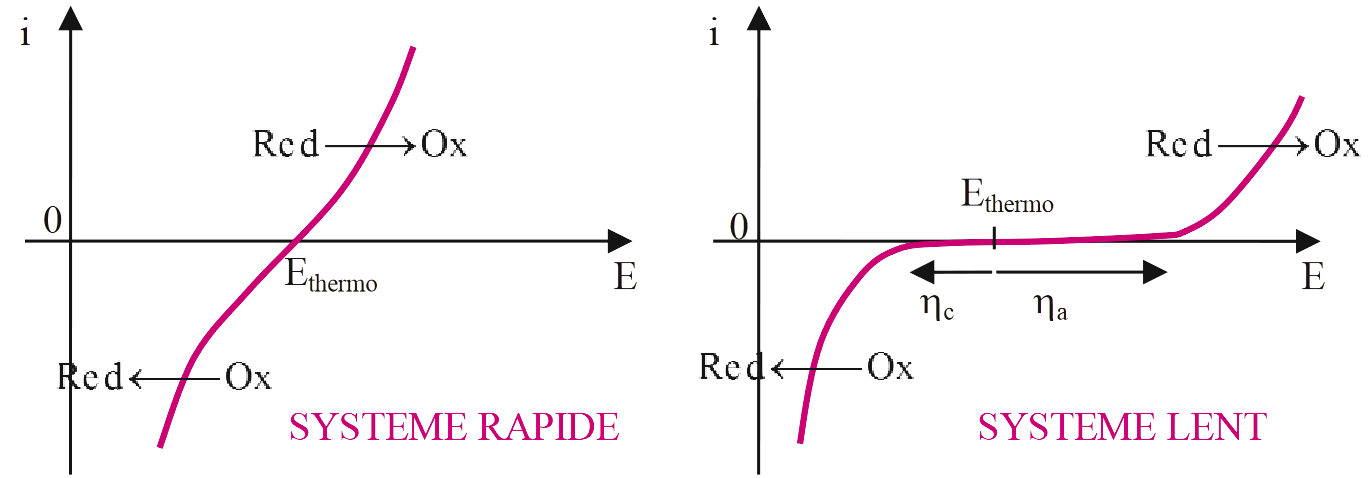
\includegraphics[width=\linewidth]{chimie/i-E/iE-cours.png}
~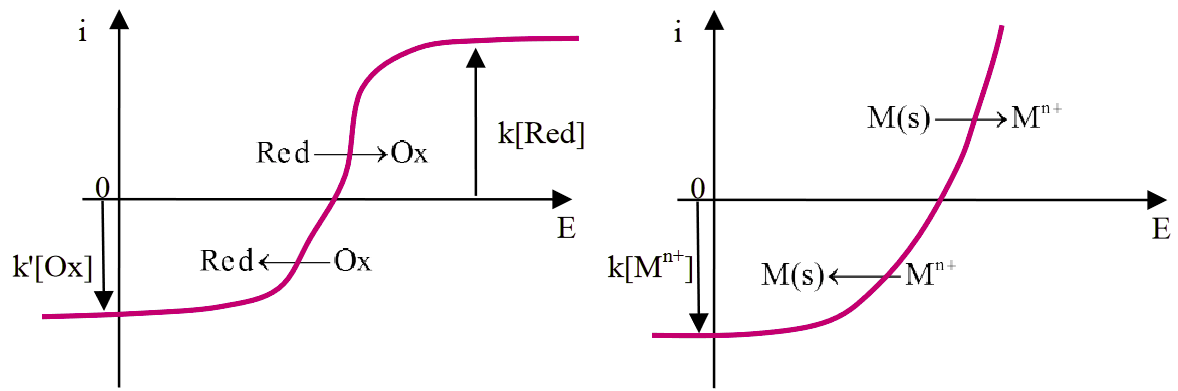
\includegraphics[width=\linewidth]{chimie/i-E/iE-cours2.png}
~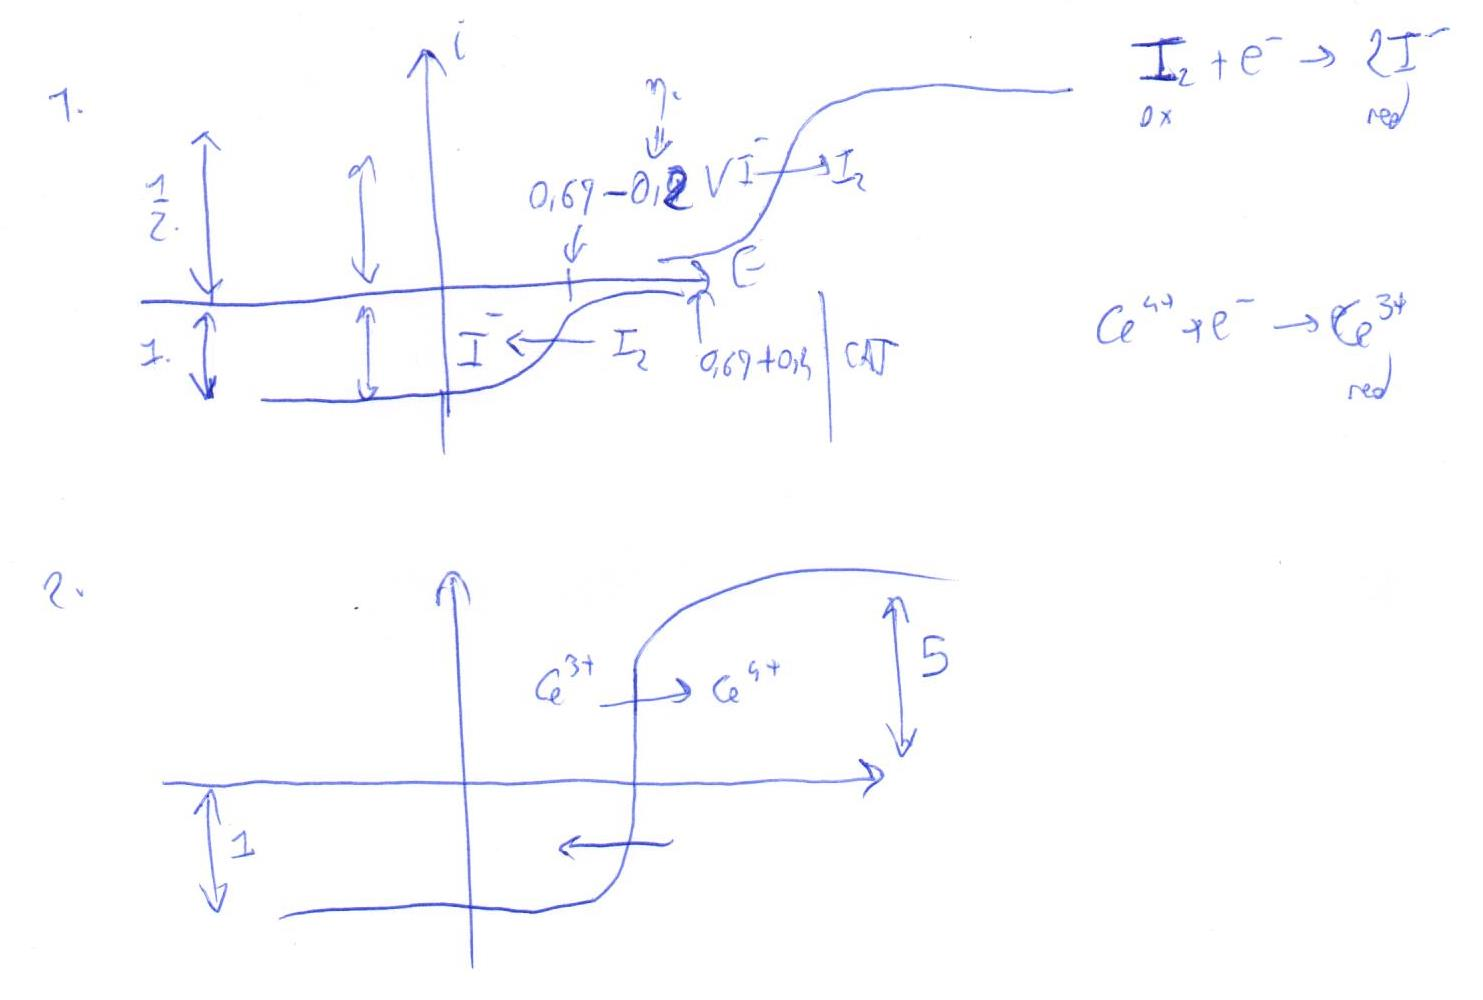
\includegraphics[width=\linewidth]{chimie/i-E/iE-corr.jpg}

\end{solution}

\begin{exercise}{Lecture de courbes $i-E$}{1}{Spé}
{Oxydoréduction, Courbes intensité potentiel}{bermu}

\textsf{Question de cours :} Interpréter quantitativement l’allure des courbes courant-tension suivantes :
\begin{questions}
    \question \hfill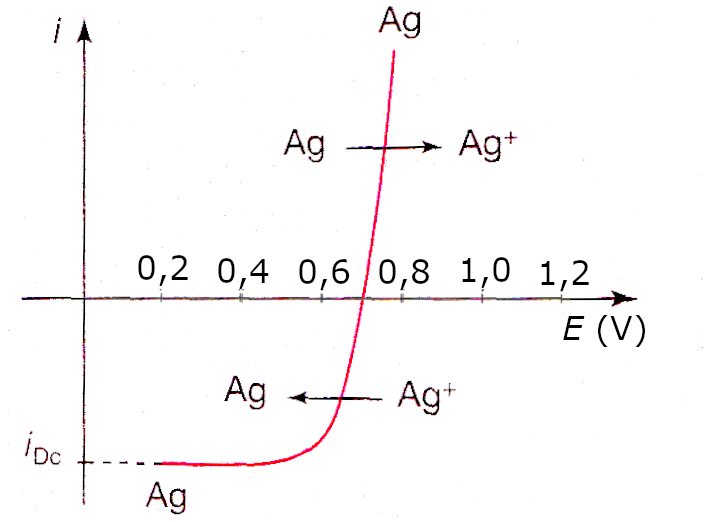
\includegraphics[valign=t,scale=1.5]{chimie/i-E/iE-2.png}\hfill ~
    
    \textsf{Données :} $[\mathrm{Ag^+}] = \SI{1e-2}{mol.L^{-1}}$, $E^\circ\qty\big(\mathrm{Ag^+_{(aq)}/Ag_{(s)}}) = \SI{0.80}{V}$.
    \question \hfill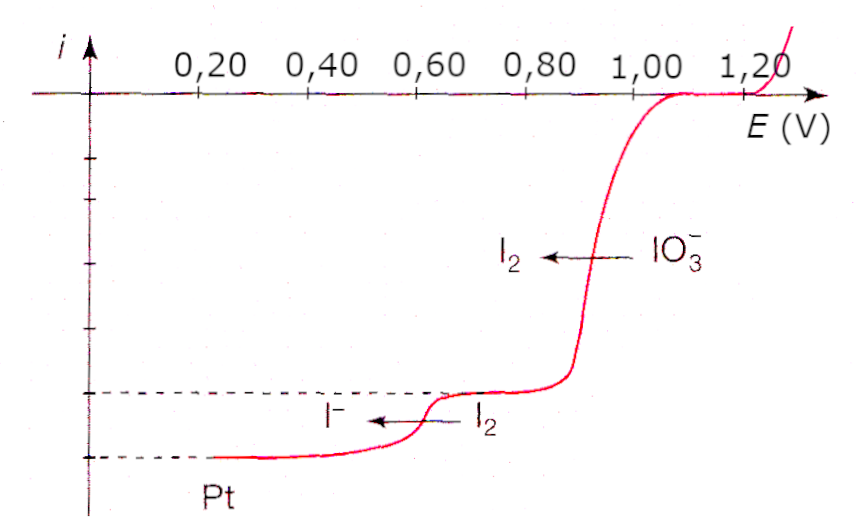
\includegraphics[valign=t,scale=1.5]{chimie/i-E/iE-1.png}\hfill ~

    \textsf{Données :} $E^\circ\qty\big(\mathrm{I_{2,(aq)}/I^-_{(aq)}}) = \SI{0.54}{V}$, $E^\circ\qty\big(\mathrm{IO^-_{3,(aq)}/I_{2,(aq)}}) = \SI{1.19}{V}$.
\end{questions}

\end{exercise}

\begin{solution}

\paragraph{Pistes :}

\begin{questions}
    \question~
        \begin{parts}
            \part Pourquoi n’observe-t-on pas de palier de diffusion anodique pour le système $\mathrm{Ag^+_{(aq)}/Ag_{(s)}}$ ?
            \part Vérifier numériquement la valeur du potentiel à l’équilibre.
            \part Ce système est-il rapide ou lent ?
        \end{parts}
    \question~
        \begin{parts}
            \part Pourquoi observe-t-on des vagues de réduction de hauteur différente ?
            \part Prévoir l’allure de la courbe d’oxydation d’une solution d’iodure sur platine.
        \end{parts}
\end{questions}

\end{solution}